% commandes
\newcommand{\notion}[1]{\textcolor{vert_fonce}{\textit{#1}}}
\newcommand{\mb}[1]{\mathbb{#1}}
\newcommand{\mc}[1]{\mathcal{#1}}
\newcommand{\mr}[1]{\mathrm{#1}}
\newcommand{\code}[1]{\texttt{#1}}
\newcommand{\ccode}[1]{\texttt{|#1|}}
\newcommand{\ov}[1]{\overline{#1}}
\newcommand{\abs}[1]{|#1|}
\newcommand{\rev}[1]{\texttt{reverse(#1)}}
\newcommand{\crev}[1]{\texttt{|reverse(#1)|}}

\newcommand{\ie}{\textit{i.e.} }

\newcommand{\N}{\mathbb{N}}
\newcommand{\R}{\mathbb{R}}
\newcommand{\C}{\mathbb{C}}
\newcommand{\K}{\mathbb{K}}
\newcommand{\Z}{\mathbb{Z}}

\newcommand{\A}{\mathcal{A}}
\newcommand{\bigO}{\mathcal{O}}
\renewcommand{\L}{\mathcal{L}}

\newcommand{\rg}[0]{\mathrm{rg}}
\newcommand{\re}[0]{\mathrm{Re}}
\newcommand{\im}[0]{\mathrm{Im}}
\newcommand{\cl}[0]{\mathrm{cl}}
\newcommand{\grad}[0]{\vec{\mathrm{grad}}}
\renewcommand{\div}[0]{\mathrm{div}\,}
\newcommand{\rot}[0]{\vec{\mathrm{rot}}\,}
\newcommand{\vnabla}[0]{\vec{\nabla}}
\renewcommand{\vec}[1]{\overrightarrow{#1}}
\newcommand{\mat}[1]{\mathrm{Mat}_{#1}}
\newcommand{\matrice}[1]{\mathcal{M}_{#1}}
\newcommand{\sgEngendre}[1]{\left\langle #1 \right\rangle}
\newcommand{\gpquotient}[1]{\mathbb{Z} / #1\mathbb{Z}}
\newcommand{\norme}[1]{||#1||}
\renewcommand{\d}[1]{\,\mathrm{d}#1}
\newcommand{\adh}[1]{\overline{#1}}
\newcommand{\intint}[2]{\llbracket #1 ,\, #2 \rrbracket}
\newcommand{\seg}[2]{[#1\, ; \, #2]}
\newcommand{\scal}[2]{( #1 | #2 )}
\newcommand{\distance}[2]{\mathrm{d}(#1,\,#2)}
\newcommand{\inte}[2]{\int_{#1}^{#2}}
\newcommand{\somme}[2]{\sum_{#1}^{#2}}
\newcommand{\deriveref}[4]{\biggl( \frac{\text{d}^{#1}#2}{\text{d}#3^{#1}} \biggr)_{#4}}





\documentclass{article}
\usepackage{amsmath,amssymb,mathtools}
\usepackage{xcolor}
\usepackage{enumitem}
\usepackage{multicol}
\usepackage{changepage}
\usepackage{stmaryrd}
\usepackage{graphicx}
\usepackage[framemethod=tikz]{mdframed}
\usepackage{tikz,pgfplots}
\pgfplotsset{compat=1.18}

% physique
\renewcommand*{\overrightarrow}[1]{\vbox{\halign{##\cr 
  \tiny\rightarrowfill\cr\noalign{\nointerlineskip\vskip1pt} 
  $#1\mskip2mu$\cr}}}
  
\definecolor{oranges}{RGB}{255, 242, 230}
\definecolor{rouges}{RGB}{255, 230, 230}
\definecolor{rose}{RGB}{255, 204, 204}

% maths - info
\definecolor{rouge_fonce}{RGB}{204, 0, 0}
\definecolor{rouge}{RGB}{255, 0, 0}
\definecolor{bleu_fonce}{RGB}{0, 0, 255}
\definecolor{vert_fonce}{RGB}{0, 69, 33}
\definecolor{vert}{RGB}{0,255,0}

\definecolor{orange_foncee}{RGB}{255, 153, 0}
\definecolor{myrtille}{RGB}{225, 225, 255}
\definecolor{mayonnaise}{RGB}{255, 253, 233}
\definecolor{magenta}{RGB}{224, 209, 240}
\definecolor{pomme}{RGB}{204, 255, 204}
\definecolor{mauve}{RGB}{255, 230, 255}


% Cours

\newmdenv[
  nobreak=true,
  topline=true,
  bottomline=true,
  rightline=true,
  leftline=true,
  linewidth=0.5pt,
  linecolor=black,
  backgroundcolor=mayonnaise,
  innerleftmargin=10pt,
  innerrightmargin=10pt,
  innertopmargin=5pt,
  innerbottommargin=5pt,
  skipabove=\topsep,
  skipbelow=\topsep,
]{boite_definition}

\newmdenv[
  nobreak=true,
  topline=true,
  bottomline=true,
  rightline=true,
  leftline=true,
  linewidth=0.5pt,
  linecolor=white,
  backgroundcolor=white,
  innerleftmargin=10pt,
  innerrightmargin=10pt,
  innertopmargin=5pt,
  innerbottommargin=5pt,
  skipabove=\topsep,
  skipbelow=\topsep,
]{boite_exemple}

\newmdenv[
  nobreak=true,
  topline=true,
  bottomline=true,
  rightline=true,
  leftline=true,
  linewidth=0.5pt,
  linecolor=black,
  backgroundcolor=magenta,
  innerleftmargin=10pt,
  innerrightmargin=10pt,
  innertopmargin=5pt,
  innerbottommargin=5pt,
  skipabove=\topsep,
  skipbelow=\topsep,
]{boite_proposition}

\newmdenv[
  nobreak=true,
  topline=true,
  bottomline=true,
  rightline=true,
  leftline=true,
  linewidth=0.5pt,
  linecolor=black,
  backgroundcolor=white,
  innerleftmargin=10pt,
  innerrightmargin=10pt,
  innertopmargin=5pt,
  innerbottommargin=5pt,
  skipabove=\topsep,
  skipbelow=\topsep,
]{boite_demonstration}

\newmdenv[
  nobreak=true,
  topline=true,
  bottomline=true,
  rightline=true,
  leftline=true,
  linewidth=0.5pt,
  linecolor=white,
  backgroundcolor=white,
  innerleftmargin=10pt,
  innerrightmargin=10pt,
  innertopmargin=5pt,
  innerbottommargin=5pt,
  skipabove=\topsep,
  skipbelow=\topsep,
]{boite_remarque}


\newenvironment{definition}[2]
{
    \vspace{15pt}
    \begin{boite_definition}
    \textbf{\textcolor{rouge}{Définition #1}}
    \if\relax\detokenize{#2}\relax
    \else
        \textit{ - #2}
    \fi \\ \\
}
{
    \end{boite_definition}
    
}

\newenvironment{exemple}[2]
{
    \vspace{15pt}
    \begin{boite_exemple}
    \textbf{\textcolor{bleu_fonce}{Exemple #1}}
    \if\relax\detokenize{#2}\relax
    \else
        \textit{ - #2}
    \fi \\ \\ 
}
{   
    \end{boite_exemple}
    
}

\newenvironment{proposition}[2]
{
    \vspace{15pt}
    \begin{boite_proposition}
    \textbf{\textcolor{rouge}{Proposition #1}}
    \if\relax\detokenize{#2}\relax
    \else
        \textit{ - #2}
    \fi \\ \\
}
{
    \end{boite_proposition}
    
}

\newenvironment{theoreme}[2]
{
    \vspace{15pt}
    \begin{boite_proposition}
    \textbf{\textcolor{rouge}{Théorème #1}} 
    \if\relax\detokenize{#2}\relax
    \else
        \textit{ - #2}
    \fi \\ \\
}
{
    \end{boite_proposition}
    
}

\newenvironment{demonstration}
{
    \vspace{15pt}
    \begin{boite_demonstration}
    \textbf{\textcolor{rouge}{Démonstration}}\\ \\
}
{
    \end{boite_demonstration}
    
}

\newenvironment{remarque}[2]
{
    \vspace{15pt}
    \begin{boite_remarque}
    \textbf{\textcolor{bleu_fonce}{Remarque #1}}
    \if\relax\detokenize{#2}\relax
    \else
        \textit{ - #2}
    \fi \\ \\   
}
{  
    \end{boite_remarque}
    
}



%Corrections
\newmdenv[
  nobreak=true,
  topline=true,
  bottomline=true,
  rightline=true,
  leftline=true,
  linewidth=0.5pt,
  linecolor=black,
  backgroundcolor=mayonnaise,
  innerleftmargin=10pt,
  innerrightmargin=10pt,
  innertopmargin=5pt,
  innerbottommargin=5pt,
  skipabove=\topsep,
  skipbelow=\topsep,
]{boite_question}


\newenvironment{question}[2]
{
    \vspace{15pt}
    \begin{boite_question}
    \textbf{\textcolor{rouge}{Question #1}}
    \if\relax\detokenize{#2}\relax
    \else
        \textit{ - #2}
    \fi \\ \\
}
{
    \end{boite_question}
    
}

% Cours

\newmdenv[
  nobreak=false,
  topline=true,
  bottomline=true,
  rightline=true,
  leftline=true,
  linewidth=0.5pt,
  linecolor=black,
  backgroundcolor=mayonnaise,
  innerleftmargin=10pt,
  innerrightmargin=10pt,
  innertopmargin=5pt,
  innerbottommargin=5pt,
  skipabove=\topsep,
  skipbelow=\topsep,
]{boite_definition_break}

\newmdenv[
  nobreak=false,
  topline=true,
  bottomline=true,
  rightline=true,
  leftline=true,
  linewidth=0.5pt,
  linecolor=white,
  backgroundcolor=white,
  innerleftmargin=10pt,
  innerrightmargin=10pt,
  innertopmargin=5pt,
  innerbottommargin=5pt,
  skipabove=\topsep,
  skipbelow=\topsep,
]{boite_exemple_break}

\newmdenv[
  nobreak=false,
  topline=true,
  bottomline=true,
  rightline=true,
  leftline=true,
  linewidth=0.5pt,
  linecolor=black,
  backgroundcolor=magenta,
  innerleftmargin=10pt,
  innerrightmargin=10pt,
  innertopmargin=5pt,
  innerbottommargin=5pt,
  skipabove=\topsep,
  skipbelow=\topsep,
]{boite_proposition_break}

\newmdenv[
  nobreak=false,
  topline=true,
  bottomline=true,
  rightline=true,
  leftline=true,
  linewidth=0.5pt,
  linecolor=black,
  backgroundcolor=white,
  innerleftmargin=10pt,
  innerrightmargin=10pt,
  innertopmargin=5pt,
  innerbottommargin=5pt,
  skipabove=\topsep,
  skipbelow=\topsep,
]{boite_demonstration_break}

\newmdenv[
  nobreak=false,
  topline=true,
  bottomline=true,
  rightline=true,
  leftline=true,
  linewidth=0.5pt,
  linecolor=white,
  backgroundcolor=white,
  innerleftmargin=10pt,
  innerrightmargin=10pt,
  innertopmargin=5pt,
  innerbottommargin=5pt,
  skipabove=\topsep,
  skipbelow=\topsep,
]{boite_remarque_break}


\newenvironment{definition_break}[2]
{
    \vspace{15pt}
    \begin{boite_definition_break}
    \textbf{\textcolor{rouge}{Définition #1}}
    \if\relax\detokenize{#2}\relax
    \else
        \textit{ - #2}
    \fi \\ \\
}
{
    \end{boite_definition_break}
    
}

\newenvironment{exemple_break}[2]
{
    \vspace{15pt}
    \begin{boite_exemple_break}
    \textbf{\textcolor{bleu_fonce}{Exemple #1}}
    \if\relax\detokenize{#2}\relax
    \else
        \textit{ - #2}
    \fi \\ \\ 
}
{   
    \end{boite_exemple_break}
    
}

\newenvironment{proposition_break}[2]
{
    \vspace{15pt}
    \begin{boite_proposition_break}
    \textbf{\textcolor{rouge}{Proposition #1}}
    \if\relax\detokenize{#2}\relax
    \else
        \textit{ - #2}
    \fi \\ \\
}
{
    \end{boite_proposition_break}
    
}

\newenvironment{theoreme_break}[2]
{
    \vspace{15pt}
    \begin{boite_proposition_break}
    \textbf{\textcolor{rouge}{Théorème #1}} 
    \if\relax\detokenize{#2}\relax
    \else
        \textit{ - #2}
    \fi \\ \\
}
{
    \end{boite_proposition_break}
    
}

\newenvironment{demonstration_break}
{
    \vspace{15pt}
    \begin{boite_demonstration_break}
    \textbf{\textcolor{rouge}{Démonstration}}\\ \\
}
{
    \end{boite_demonstration_break}
    
}

\newenvironment{remarque_break}[2]
{
    \vspace{15pt}
    \begin{boite_remarque}
    \textbf{\textcolor{bleu_fonce}{Remarque #1}}
    \if\relax\detokenize{#2}\relax
    \else
        \textit{ - #2}
    \fi \\ \\   
}
{  
    \end{boite_remarque}
    
}



%Corrections
\newmdenv[
  nobreak=false,
  topline=true,
  bottomline=true,
  rightline=true,
  leftline=true,
  linewidth=0.5pt,
  linecolor=black,
  backgroundcolor=mayonnaise,
  innerleftmargin=10pt,
  innerrightmargin=10pt,
  innertopmargin=5pt,
  innerbottommargin=5pt,
  skipabove=\topsep,
  skipbelow=\topsep,
]{boite_question_break}


\newenvironment{question_break}[2]
{
    \vspace{15pt}
    \begin{boite_question_break}
    \textbf{\textcolor{rouge}{Question #1}}
    \if\relax\detokenize{#2}\relax
    \else
        \textit{ - #2}
    \fi \\ \\
}
{
    \end{boite_question_break}
    
}

\newenvironment{enumeratebf}{
    \begin{enumerate}[label=\textbf{\arabic*.}]
}
{
    \end{enumerate}
}

\begin{document}
\begin{adjustwidth}{-3cm}{-3cm}


\setcounter{section}{6}
\section{Arbres}
Nous avons jusqu'à présent étudié des structures de données séquentielles (piles, files, tables de hachage, etc.). Dans ce chapitre, on étudie des structures de données hiérarchiques. \\
On peut définir la structure d'\notion{arbre} de différentes façons, avec quelques subtilités, ce qui offre une certaine souplesse et permet de s'adapter au problème étudié. \textbf{Il convient d'être particulièrement vigilant à la lecture des sujets proposés pour identifier correctement la structure attendue}.
\subsection{Arbres binaires}

\begin{definition}{7.1}{arbre binaire}
    Un \notion{arbre binaire} est un ensemble (éventuellement vide) de \notion{nœuds} et est défini de manière inductive. Un arbre binaire est : \begin{itemize}
        \item Ou bien \notion{l'arbre vide}
        \item Ou bien constitué d'un nœud $R$, appelé \notion{racine}, et de deux \notion{sous-arbres} binaires. Si existence, on appelle \notion{fils gauche} (resp. \notion{fils droit}) du nœud $R$ la racine du sous-arbre gauche (resp. droit). \\ \textit{Voir Figure 1}
    \end{itemize}
\end{definition}

\begin{remarque}{7.2}{à propos de la précédente définition}
    Dans cette définition, si on permute les sous-arbres gauche et droit, on obtient un arbre différent. Ainsi, les deux arbres représentés ci-dessous sont deux arbres distincts : 
    \begin{center}
    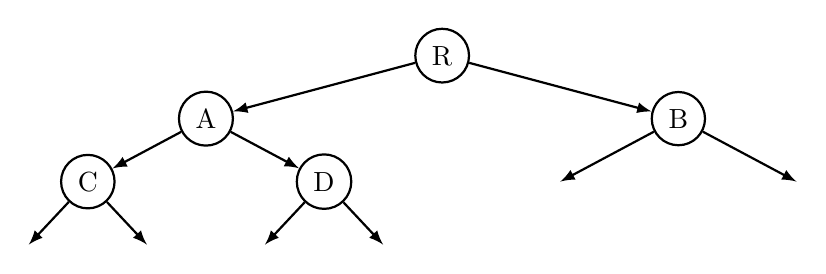
\begin{tikzpicture}[every node/.style={draw,thick,circle}, every path/.style={thick, ->, >=latex},%
        level distance=.8cm, level 1/.style={sibling distance = 6cm}, level 2/.style = {sibling distance = 3cm}, level 3/.style = {sibling distance = 1.5cm}, level 4/.style = {sibling distance = .8cm}]
        \node {R}
        child { node {A}
                child { node {C}
                        child {}
                        child {}
                }
                child { node {D}
                        child {}
                        child {}
                }
        }
        child { node {B}
                child {}
                child {}
        };
    \end{tikzpicture}
\end{center}
    \centering{V/S}
    \begin{center}
    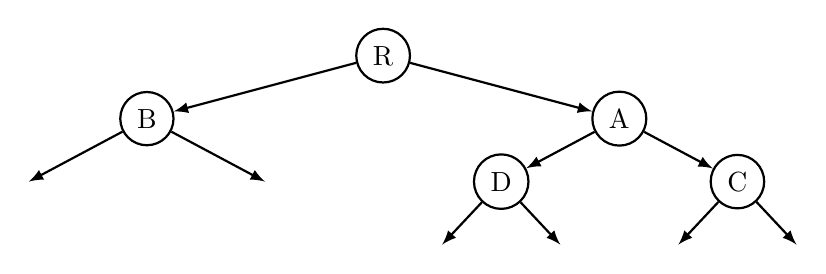
\begin{tikzpicture}[every node/.style={draw,thick,circle}, every path/.style={thick, ->, >=latex},%
        level distance=.8cm, level 1/.style={sibling distance = 6cm}, level 2/.style = {sibling distance = 3cm}, level 3/.style = {sibling distance = 1.5cm}, level 4/.style = {sibling distance = .8cm}]
        \node {R}
        child { node {B}
                child {}
                child {}
        }
        child { node {A}
                child { node {D}
                        child {}
                        child {}}
                child { node {C}
                        child {}
                        child {}
                }
        };
    \end{tikzpicture}
\end{center}
\end{remarque}

\begin{definition}{7.3}{feuille, père, arête, taille}
    \begin{itemize}
        \item Une \notion{feuille} est un nœud dont les sous-arbres gauche et droit sont l'arbre vide.
        \item Un nœud est le \notion{père} de ses éventuels fils. La liaison d'un père vers un fils est appelée une \notion{une arête}.
        \item Tous les nœuds d'un arbre, hormis la racine et les feuilles, sont appelés des \notion{nœuds internes}.
        \item La \notion{taille} d'un arbre est son nombre de nœuds. On note $\abs{\mc{A}}$ la taille de l'arbre $\mc{A}$
    \end{itemize}
\end{definition}

\begin{remarque}{7.4}{définition inductive de la taille d'un arbre binaire}
    \begin{itemize}
        \item La taille de l'arbre vide est nulle
        \item Un arbre binaire comportant un sous-arbre gauche de taille $n_g$ et un sous-arbre droit de taille $n_d$ est de taille $1+n_g+n_d$ 
    \end{itemize}
    
\end{remarque}

\begin{definition}{7.5}{hauteur, profondeur}
    La \notion{hauteur} d'un arbre binaire est définie inductivement : \begin{itemize}
        \item L'arbre vide est de hauteur : $-1$
        \item Un arbre binaire comportant un sous-arbre gauche de hauteur $h_g$ et un sous-arbre droit de hauteur $h_d$ est de hauteur $1+\max(h_g,h_d)$.
    \end{itemize}
    La \notion{profondeur} d'un nœud est la distance de celui-ci à la racine (si existence). La hauteur d'un arbre est alors la profondeur maximale de ses neuds, et donc la profondeur maximale de ses feuilles.
\end{definition}

\begin{remarque}{7.6}{notion d'étiquettes}
    Les nœuds et les arêtes d'un arbre peuvent porter des \notion{étiquettes} : on leur associe alors une valeur. 
\end{remarque}

\begin{exemple}{7.7}{concernant les précédentes définitions}
    Considérons l'arbre binaire suivant:
    \begin{center}
    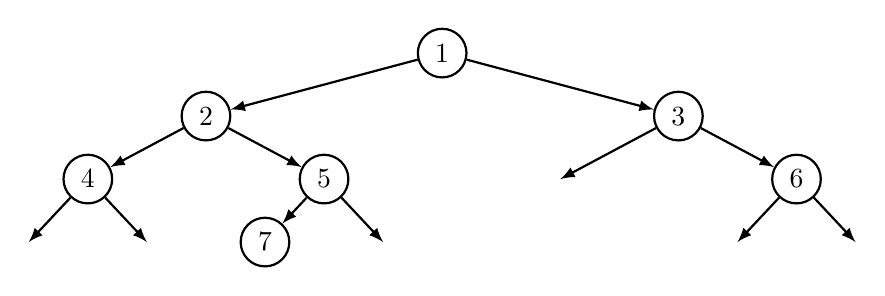
\begin{tikzpicture}[every node/.style={draw,thick,circle}, every path/.style={thick, ->, >=latex},%
        level distance=.8cm, level 1/.style={sibling distance = 6cm}, level 2/.style = {sibling distance = 3cm}, level 3/.style = {sibling distance = 1.5cm}, level 4/.style = {sibling distance = .8cm}]
        \node {1}
        child { node {2}
                child { node {4}
                        child {}
                        child {}
                }
                child { node {5}
                        child { node {7}}
                        child {}
                }
        }
        child { node {3}
                child {}
                child { node {6}
                        child {}
                        child {}
                }
        };
    \end{tikzpicture}
\end{center}
    \begin{itemize}
        \item Il s'agit d'un arbre binaire de taille 7, (il comporte sept nœuds étiquetés de 1 à 7) et de hauteur 3.
        \item Sa racine est le nœud 1, de profondeur 0.
        \item Les nœuds 2 et 3 sont de profondeur 1.
        \item Les nœuds 4, 5 et 6 sont de profondeur 2.
        \item Le nœud 7 est de profondeur 3.
        \item Ses feuilles sont les nœuds 4, 6 et 7.
        \item Ses nœuds internes sont les nœuds 2, 3 et 5.
        \item Le nœud 2 comporte 2 fils : le nœud 4 (son fils gauche) et le nœud 5 (son fils droit).
        \item Le nœud 3 est le père du nœud 6.
    \end{itemize}
\end{exemple}

\begin{exemple}{7.8}{implémentation en Ocaml}
    Les arbres binaires étiquetés peuvent être implémentés en Ocaml en définissant le type suivant :
    \begin{verbatim}
        type 'a bintree = Vide | Noeud of 'a * 'a bintree 'a * bintree
    \end{verbatim}
    On déclare alors l'arbre de l'exemple précédent comme ceci : 
    \begin{verbatim}
        let a = Noeud(1,
            Noeud(2,
                Noeud(4,Vide,Vide),
                Noeud(5,
                    Noeud(7,Vide,Vide),
                    Vide)),
            Noeud(3,
                Vide,
                Noeud(6, Vide, Vide)))
    \end{verbatim}
    La fonction suivante permet de déterminer la taille d'un arbre binaire.
    \begin{verbatim}
    let taille arbre = match arbre with
        |Vide -> 0
        |Noeud (e, g, d) -> 1 + taille g + taille d

    let () = print_int (taille a ; print_string "\n")
    \end{verbatim}
\end{exemple}

\begin{definition}{7.9}{arbres complets}
    Un arbre binaire est dit \notion{complet} si l'une des propriétés est vraie : \begin{itemize}
        \item il est vide
        \item ses sous-abres gauche et droit sont complets, et de même hauteur.
    \end{itemize}
    
\end{definition}

\begin{proposition}{7.10}{lien entre hauteur et taille pour un arbre complet}
    Tout arbre binaire complet de hauteur $h$ possède exactement $2^{h+1} - 1$ noeuds.
\end{proposition}

\begin{demonstration}
    On rappelle que pour tout arbre $\mc{A}$ on note $|\mc{A}|$ sa taille, i.e. son nombre de nœuds. \\ Montrons par récurrence sur $h$ que pour tout arbre complet $\mc{A}$ de hauteur $h$, $|\mc{A}| = 2^{k+1} - 1$. \begin{itemize}
        \item L'unique arbre de hauteur $-1$ est l'arbre vide, qui est bien de taille $0 = 2^{-1+1} - 1$.
        \item Soit $h \in \mb{N}$ fixé. On suppose que tout arbre binaire complet de hauteur $h-1$ est de taille $2^k - 1$. \\ On considère un arbre binaire complet $\mc{A}$ de hauteur $h$. Par définition, $\mc{A}$ possède un sous-arbre gauche $\mc{A}_g$ et un sous-arbre droit $\mc{A}_d$, tous deux complets et de hauteur $h-1$. Alors, \begin{align*}
            |\mc{A}| &= 1 + |\mc{A}_g| + |\mc{A}_d| \\
            &= 1 + 2^k -1 + 2^k - 1 &&\text{Hypothèse de récurrence} \\
            &= 2^{k+1} - 1
        \end{align*}
    \end{itemize}
    Par principe de récurrence, le prédicat est vrai pour tout arbre $\mathcal{A}$ de hauteur h $\in \mathbb{N}$ $\cup$ {$-1$}
\end{demonstration}

\begin{exemple}{7.11}{implémentation en C}
    En C, on peut définir une structure d'arbre binaire dans laquelle on stocke la taille de l'arbre :
    \begin{verbatim}{C}
        struct Arbrebin{
            int taille;
            struct Arbrebin* gauche;
            struct Arbrebin* droit;
        };
        type def struct Arbrebin arbrebin;
    \end{verbatim}
    L'arbre vide est représenté par le pointeur \code{NULL}. Pour pouvoir accéder à la taille, y compris de l'arbre vide, on implémente une fonction taille : 
    \begin{verbatim}{C}
        int taille(arbrebin* a){
            if (a == NULL){
                return 0;
            }
            return a->taille;
        }
    \end{verbatim}
    On crée alors un abre binaire quelconque en assemblant ses sous-arbres gauche et droit : 
    \begin{verbatim}{C}
        arbrebin* assemble_arbrebin(arbrebin* ssArbre_g, arbre* ssArbre_d){
            arbrebin* a = malloc(sizeof (arbrebin));
            assert(a != NULL);
            a->gauche = ssArbre_g;
            a->droite = ssArbre_d;
            a->taille = ssArbre_g->taille + ssArbre_d->taille + 1;
        }
    \end{verbatim}
    On pense également à créer un destructeur pour pouvoir libérer la mémoi allouée sur le tas : 
    \begin{verbatim}{C}
        void libere_arbre(arbrebin* a){
            if (a != NULL){
                libere_arbrebin(a->gauche);
                libere_arbrebin(a->droit);
                free(a);
            }
        }
    \end{verbatim}
    Pour créer une feuille,
    \begin{verbatim}{C}
        arbrebin* feuille = assemble_arbrebin(NULL,NULL);
    \end{verbatim}
    La fonction suivante permet de tester si un arbre binaire est complet ou non : 
    \begin{verbatim}{C}
        bool est_complet(arbrebin* a){
            if (a == NULL){return true;} // arbre vide
        }
        return taille(a->gauche) == taille(a->droit) && est_complet(a->gauche) && est_complet(a->droit)
    \end{verbatim}
\end{exemple}

\begin{remarque}{7.12}{comparaison entre C et Ocaml}
    Dans ce précédent exemple, on représente des arbres binaires non étiquetés, mais on pouvait tout à fait ajouter un champ étiquette. Par ailleurs, en C, on a naturellement une structure mutable, ce qui permet de modifier la structure d'un arbre ou ses étiquettes. Ce n'est pas le cas en Ocaml.
\end{remarque}

\begin{exemple}{7.13}{autre structure de définition}
    Dans le cas d'un arbre binaire complet ou \notion{presque complet} (tous les niveaux de profondeur sont remplis sauf éventuellement le dernier qui est rempli de gauche à droite), on peut également utiliser une structure de tableau. Pour cela, il suffit de numéroter les nœuds de haut en bas et de gauche à droite, à partir de 0, en remarquant que: 
    \begin{itemize}
        \item S'il existe, le fils gauche du nœud d'étiquette $i$ porte le numéro $2i + 1$
        \item S'il existe, le fils gauche du nœud d'étiquette $i$ porte le numéro $2i + 2$
        \item Le père du noeud d'étiquette $i$ (sauf pour la racine qui n'a pas de père) porte le numéro $\left\lfloor \frac{i-1}{2}\right\rfloor $
    \end{itemize}
    \begin{center}
    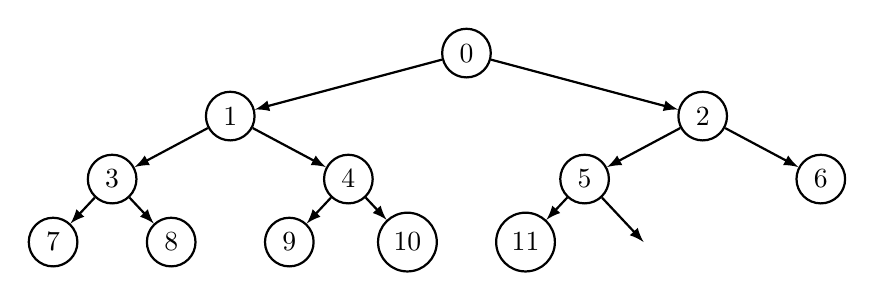
\begin{tikzpicture}[every node/.style={draw,thick,circle}, every path/.style={thick, ->, >=latex},%
        level distance=.8cm, level 1/.style={sibling distance = 6cm}, level 2/.style = {sibling distance = 3cm}, level 3/.style = {sibling distance = 1.5cm}, level 4/.style = {sibling distance = .8cm}]
        \node {0}
        child { node {1}
                child { node {3}
                        child { node {7}}
                        child { node {8}}
                }
                child { node {4}
                        child { node {9}}
                        child { node {10}}
                }
        }
        child { node {2}
                child { node {5}
                        child { node {11}}
                        child {}
                        }
                child { node {6}}
        };
    \end{tikzpicture}
\end{center}
    
    En C, pour manipuler de tels arbres, on peut utiliser la structure suivante :
    \begin{verbatim}{C}
        typedef struct ArbreBC{
            int taille;
            int* etiquettes; //ou un autre type, en fonction des étiquettes
        } arbreBC;

        arbreBC* cree_arbreBC(int nb_noeuds){
            arbreBC* a = malloc(sizeof (arbreBC));
            assert(a != NULL); //allocation réussie
            a->taille = nb_noeuds;
            a->etiquettes = malloc(nb_noeuds * sizeof (int)); // attention, étiquettes non renseignées.
            assert(a->etiquettes != NULL);
            return a;
        }

        void libere_arbreBC(arbreBC* a){
            if (a != NULL){
                free(a->etiquettes);
                free(a);
            }
        }
    \end{verbatim}
\end{exemple}

 \begin{remarque}{7.14}{}
    Dans la littérature on peut trouver plusieurs définitions, parfois contradictoires, d'arbres binaires complets ou parfaits. \textbf{Là encore, il convient de bien lire les énoncés !}
 \end{remarque}

 \subsection{Parcours d'arbres binaires}
 Parcourir un arbre signifie parcourir l'ensemble de ses noeuds (par exemple dans le but de rechercher un élément particulier, éventuellement pour le modifier), une et une seule fois. Il existe plusieurs façons de parcourir un arbre binaire, mais nous allons décrire les parcours en profondeur et en largeur (dans les deux cas, le parcours s'effectue de gauche à droite).

 \subsubsection{Parcours en profondeur}
 \begin{definition}{7.15}{parcours infixe, postfixe, préfixe}
    On effecue un \notion{parcours en profondeur} lorsqu'on parcourt les noeuds en descendant le plus profondément possible dans l'arbre avant de remonter pour parcourir le reste de l'arbre. \\Il existe 3 parcours classiques en profondeur : \begin{itemize}
        \item le \notion{parcours préfixe} traite chaque noeud avant de parcourir ses deux sous-arbres (gauche puis droit).
        \item le \notion{parcours infixe} traite chaque noeud entre le parcours du sous-arbres gauche et celui du sous-arbre droit.
        \item le \notion{parcours postfixe} traite chaque noeud après avoir parcouru ses deux sous-arbres (le gauche puis le droit).
    \end{itemize}
 \end{definition}

\begin{exemple}{7.16}{application des parcours en profondeur}
    \begin{center}
    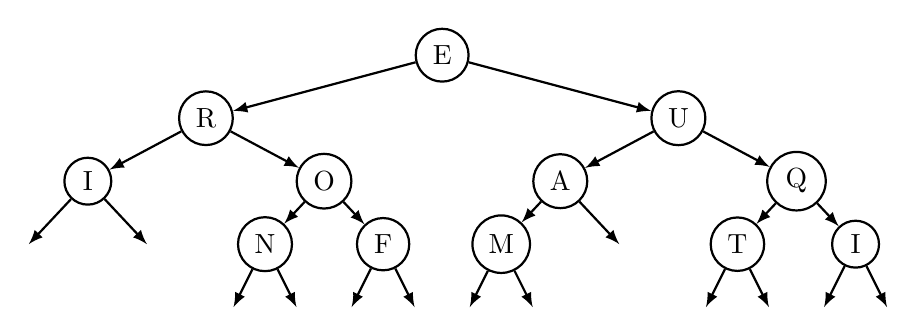
\begin{tikzpicture}[every node/.style={draw,thick,circle}, every path/.style={thick, ->, >=latex},%
        level distance=.8cm, level 1/.style={sibling distance = 6cm}, level 2/.style = {sibling distance = 3cm}, level 3/.style = {sibling distance = 1.5cm}, level 4/.style = {sibling distance = .8cm}]
        \node {E}
        child { node {R}
                child { node {I}
                        child {}
                        child {}
                }
                child { node {O}
                        child { node {N}
                                child {}
                                child {}
                        }
                        child { node {F}
                                child {}
                                child {}
                        }
                }
        }
        child { node {U}
                child { node {A}
                        child { node {M}
                                child {}
                                child {}
                        }
                        child {}}
                child { node {Q}
                        child { node {T}
                                child {}
                                child {}
                        }
                        child { node {I}
                                child {}
                                child {}
                        }
                }
        };
    \end{tikzpicture}
\end{center}
    Si on parcourt l'arbre binaire ci-dessus pour afficher l'étiquette de chaque noeud, on obtient : \begin{itemize}
        \item parcours \underline{préfixe} : ERIOFUAMQTI
        \item parcours \underline{infixe} : IRNOFEMAUTQI
        \item parcours \underline{postfixe} : INFORMATIQUE
    \end{itemize}
    En reprenant le type défini dans l'exemple (7.8), cela donne :
    \begin{verbatim}
        let rec affiche_infixe(arbrebin:char bintree) =
        match arbrebin with
            | Vide -> ()
            | Noeud (e,g,d) -> affiche_infixe g;
            print_char e;
            affiche_infixe d;
    \end{verbatim}
\end{exemple}

\begin{remarque}{7.17}{compatibilité de ces parcours}
    Les parcours en profondeur sont particulièrement adaptés à la définition inductive des arbres binaires et s'implémentent avec des fonctions récursives.
\end{remarque}

\begin{remarque}{7.18}{changement de pratique}
    Maintenant que nous avons manipulé des arbres binaires en gardant en tête que chaque noeud doit avoir exactement deux sous-arbres (éventuellement vides), on peut sans ambiguïté ne plus représenter les sous-arbres vides. Cela donne pour l'exemple précédent :
    \begin{center}
    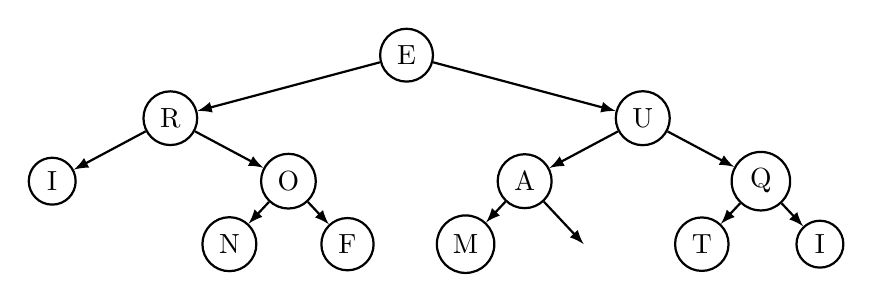
\begin{tikzpicture}[every node/.style={draw,thick,circle}, every path/.style={thick, ->, >=latex},%
        level distance=.8cm, level 1/.style={sibling distance = 6cm}, level 2/.style = {sibling distance = 3cm}, level 3/.style = {sibling distance = 1.5cm}, level 4/.style = {sibling distance = .8cm}]
        \node {E}
        child { node {R}
                child { node {I}
                }
                child { node {O}
                        child { node {N} }
                        child { node {F}}
                }
        }
        child { node {U}
                child { node {A}
                        child { node {M}}
                        child {}}
                child { node {Q}
                        child { node {T}}
                        child { node {I}}
                }
        };
    \end{tikzpicture}
\end{center}
\end{remarque}

\begin{exemple}{7.19}{cas du tri fusion}
    Lorsqu'on fait appel à une fonction récursive, avec appels multiples, on peut représenter ces appels à l'aide d'un arbre (exemple du tri fusion ci-dessous) et l'empilement des blocs d'activation dans la pile d'appels correspond alors à un  parcours \textbf{postfixe} . Ainsi les sous-arbres de chaque noeud sont bient traités  \textbf{avant} le noeud considéré.
    \begin{center}
        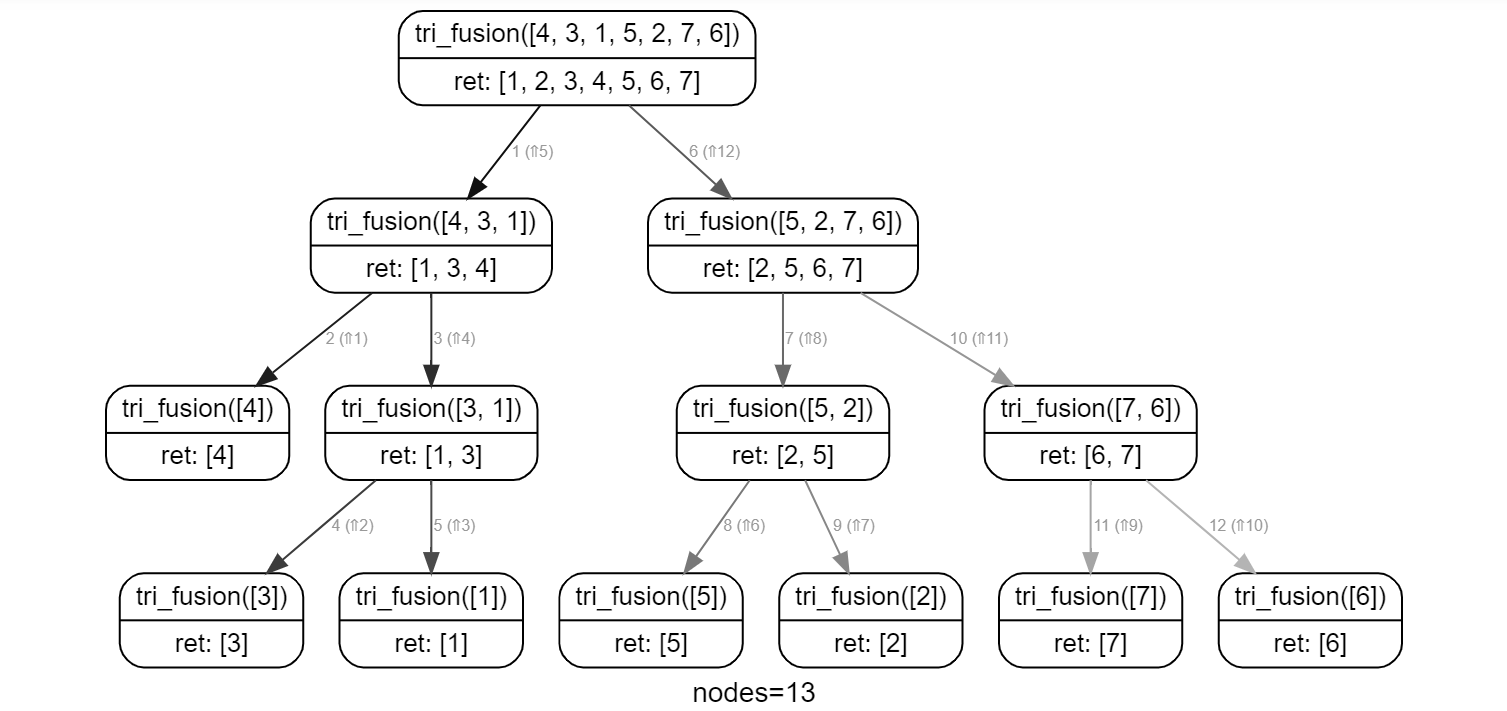
\includegraphics[scale = 0.65]{tri-fusion.png}
    \end{center}
\end{exemple}

\subsubsection{Parcours en largeur}

\begin{definition}{7.20}{parcours en largeur}
On effectue un \notion{parcours en largeur} lorsqu'on parcourt les noeuds par niveau de profondeur : on explore la racine, puis les noeuds de profondeur 1 \textbf{de gauche à droite}, puis ceux de profondeur 2, etc.
\end{definition}

\begin{exemple}{7.21}{application du parcours en largeur}
    Un parcours en largeur de l'arbre donné dans l'exemple 7.16 affiche : \\ \begin{center}ERUIOAQNFMTI\end{center}.
\end{exemple}

\begin{exemple}{7.22}{implémentation en OCaml}
    On suppose avoir défini une structure de file ainsi que les opérations élémentaires associées (voir section 5.2.3). La fonction suivante permet alors d'effectuer un parcours en largeur d'un arbre binaire : \\ \\
    \begin{verbatim}
        type a' queue = {entrants : 'a list ; sortants : 'a list}
        (* empty_queue : unit -> 'a queue
        is_empty : 'a queue -> bool
        enfile : 'a -> 'a queue -> 'a queue
        defile : 'a queue -> 'a * 'a queue *)
    
        let affiche_largeur arbrebin = 
            let rec affiche niveau suivant = match niveau with 
                (* manipule deux files d'arbres binaires :  
                    - niveau en cours d'affichage
                    - suivant : niveau suivant *)
                | f when is_empty f -> if not is_empty suivant then affiche suivant empty_queue
                | _ -> let a, file = defile niveau in 
                    begin match a with 
                        | Vide -> affiche file suivant 
                        | Noeud (e, g, d) -> 
                            print_char e; 
                            let next = enfile d (enfile g suivant) in affiche file next 
                            (* les sous-arbres vont au niveau suivant *)
                    end
            in affiche {entrants = [arbrebin]; sortants = []}
    \end{verbatim}
\end{exemple}

\begin{remarque}{7.23}{sur l'implémentation d'un arbre quasi-complet ou complet}
    On note que dans un parcours en largeur, la définition inductive des arbres n'est pas naturellement exploitable. Si, en revanche, on utilise une structure de tableau comme mentionné dans (7.13), cela revient à un parcours séquentiel du tableau.
\end{remarque}

\subsection{Arbres binaires de recherche}

\begin{definition}{7.24}{arbres binaires de recherche (ABR)}
    Un \notion{arbre binaire de recherche} (abrégé en ABR, BST (Binary Search Tree) en anglais) est un arbre binaire étiqueté tel que : \begin{itemize}
        \item l'ensemble des étiquettes est muni d'un \textbf{ordre total}
        \item pour tout noeud d'étiquette $e$, \begin{itemize}
            \item l'éventuel sous-arbre gauche comporte des noeuds étiquetés par des valeurs \underline{inférieures} à $e$
            \item l'éventuel sous-arbre droit comporte des noeuds étiquetés par des valeurs \underline{supérieures} à $e$
        \end{itemize}
    \end{itemize}
\end{definition}

\begin{exemple}{7.25}{cas de l'ordre lexicographique}
    En munissant l'ensemble des mots de l'ordre lexicographique (i.e. alphabétique), l'arbre binaire suivant est un arbre binaire de recherche :
    \begin{center}
    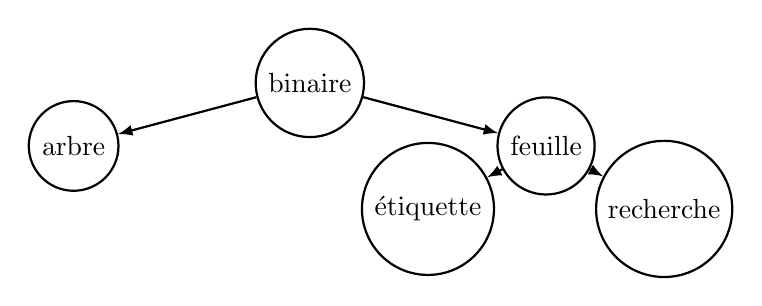
\begin{tikzpicture}[every node/.style={draw,thick,circle}, every path/.style={thick, ->, >=latex},%
        level distance=.8cm, level 1/.style={sibling distance = 6cm}, level 2/.style = {sibling distance = 3cm}, level 3/.style = {sibling distance = 1.5cm}, level 4/.style = {sibling distance = .8cm}]
        \node {binaire}
        child { node {arbre}
        }
        child { node {feuille}
                child { node {étiquette}}
                child { node {recherche}}
        };
    \end{tikzpicture}
\end{center}
\end{exemple}

\begin{exemple}{7.26}{contre-exemple d'ABR}
    L'arbre suivant n'est pas un ABR :
    \begin{center}
    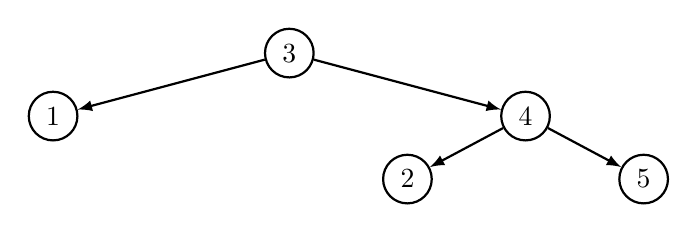
\begin{tikzpicture}[every node/.style={draw,thick,circle}, every path/.style={thick, ->, >=latex},%
        level distance=.8cm, level 1/.style={sibling distance = 6cm}, level 2/.style = {sibling distance = 3cm}, level 3/.style = {sibling distance = 1.5cm}, level 4/.style = {sibling distance = .8cm}]
        \node{3}
        child {node{1}}
        child {node{4}
            child {node{2}}
            child {node{5}}
        };
    \end{tikzpicture}
\end{center}
   
\end{exemple}

\begin{remarque}{7.27}{Définition inductive d'un ABR}
    \begin{itemize}
        \item L'arbre vide est un ABR.
        \item Un arbre binaire comportant une racine et deux sous-arbres qui sont des ABR et tel que toutes les étiquettes de son sous-arbre gauche (resp. droit) sont inférieures (resp. supérieures) à celle de sa racine est un ABR.
    \end{itemize}
\end{remarque}

\begin{proposition}{7.28}{caractérisation d'un ABR}
    Un arbre binaire étiqueté $\mc{A}$ est un ABR si et seulement si la liste des étiquettes de $\mc{A}$ obtenue par un parcours infixe de $\mc{A}$ est triée.
\end{proposition}

\begin{demonstration}
    $\implies$ On raisonne par induction structurelle sur $\mc{A}$.
    \begin{itemize}
        \item Si $\mc{A}$ est l'arbre vide, c'est immédiat.
        \item Si $\mc{A}$ est construit à partir d'une racine étiquetée par la valeur $r$, d'un sous-arbre gauche $\mc{A}_g$ et d'un sous-arbre droit $\mc{A}_d$, on suppose la propriété vraie pour les sous-arbres $\mc{A}_g$ et $\mc{A}_d$. \\ On note respectivement \code{lg} et \code{ld} les listes d'étiquettes obtenues par un parcours infixe de $\mc{A}_g$ et $\mc{A}_d$ respectivement. Par définition d'un parcours infixe, la liste \code{l} des étiquettes de $\mc{A}$ das l'ordre infixe est telle que $\code{l} = \code{lg @ [r] @ ld}$.
        \item Si $\mc{A}$ est un ABR, tous les éléments de \code{lg} sont inférieurs à l’étiquette de la racine tandis que ceux de \code{ld} sont supérieurs à \code{r}. D’autre part, $\mc{A}_g$ et $\mc{A}_d$ sont des ABR, par hypothèse d’induction, les listes \code{lg} et \code{lg} sont alors triées et on en déduit que $\code{l}=\code{lg @ [r] @ ld}$ est triée.
    \end{itemize}
    % \end{itemize} \\ \\
    % $\impliedby$
\end{demonstration}

\end{adjustwidth}
\end{document}